\documentclass[problems]{esg8022pset} 
\usepackage{amsmath}
\usepackage{amssymb}
\usepackage{enumerate}
\usepackage{graphicx}
\usepackage{hyperref}
\usepackage{mathtools}
\usepackage[per-mode=symbol,exponent-product=\cdot]{siunitx} %If this line is giving you trouble, try replacing per-mode with per
%use inter-unit-separator={}\cdot{} ?
\providecommand{\uvec}[1]{{\hat{\bf{#1}}}}
\usepackage{pgf,tikz}
\usetikzlibrary{arrows}
\usepackage{wasysym}
\usepackage{subfig}
\usepackage{wrapfig}
\makeatletter
\newcommand{\interitemtext}[1]{%
  \begin{list}{}
   {\itemindent=0mm\labelsep=0mm
   \labelwidth=0mm\leftmargin=0mm
   \addtolength{\leftmargin}{-\@totalleftmargin}}
    \item #1
  \end{list}
}
\makeatother
\renewcommand{\d}{\,d}
\providecommand{\norm}[1]{\lVert#1\rVert}

\AtBeginDocument{%
  % Appologies to any future editor on the inconsistencies in TeX code and the unnecessary braces.  I'm aggregating previously typeset problems, and didn't think it worth my time to improve the quality of TeX code in ways that won't make any difference to the typeset material. -Jason Gross (jgross@mit.edu)
}%
\classname{Physics 8.022} \semester{Spring 2011} 
\problemsetnumber{7}
\date{\today }
\duedate{Monday, March 28 at 10 \textsc {pm}}
\readingassignment{}
\problemsettitle{Magnetic Force, Special Relativity, Review}
\begin{document}
  \noindent \textbf{Review past concepts \& problems!!!}

  \noindent \textbf{Reading on complex numbers:} \url{http://web.mit.edu/sahughes/www/8.022/complex.pdf}
\section{Problem \thesection: }
  Particle $A$ with charge $q$ and mass $m_A$ is accelerated from rest by a potential difference $\Delta V$, and subsequently deflected by a uniform magnetic field into a semicircular path of radius $R$.  The direction of the magnetic field is perpendicular to the velocity of the particle.  Particle $B$ with charge $2q$ and mass $m_B$ is then accelerated from rest by the same potential difference $\Delta V$, and subsequently deflected by the same uniform magnetic field into a semicircular path of radius $2R$.  What is the ratio of the masses of the particles?
\section{Problem \thesection: }
  Let us treat the motion of an electron in a hydrogen atom classically. Suppose that an electron follows a circular orbit of radius $r$ around a proton. What is the angular frequency of the orbit $\omega$? Suppose now that a \emph{small} magnetic field perpendicular to the plane of the orbit is switched on. Assuming that the radius of the orbit does not change, calculate the shift in orbital frequency in terms of the magnitude of $B$. This is known as the ``Zeeman effect''.
\section{Problem \thesection: }
  A rod with a mass $m$ and a radius $R$ is mounted on two parallel rails of length a separated by a distance $\ell$, as shown in the figure below. The rod carries a current $I$ and rolls without slipping along the rails which are placed in a uniform magnetic field $\vec B$ directed into the page. If the rod is initially at rest, what is its speed as it leaves the rails?
  \begin{center}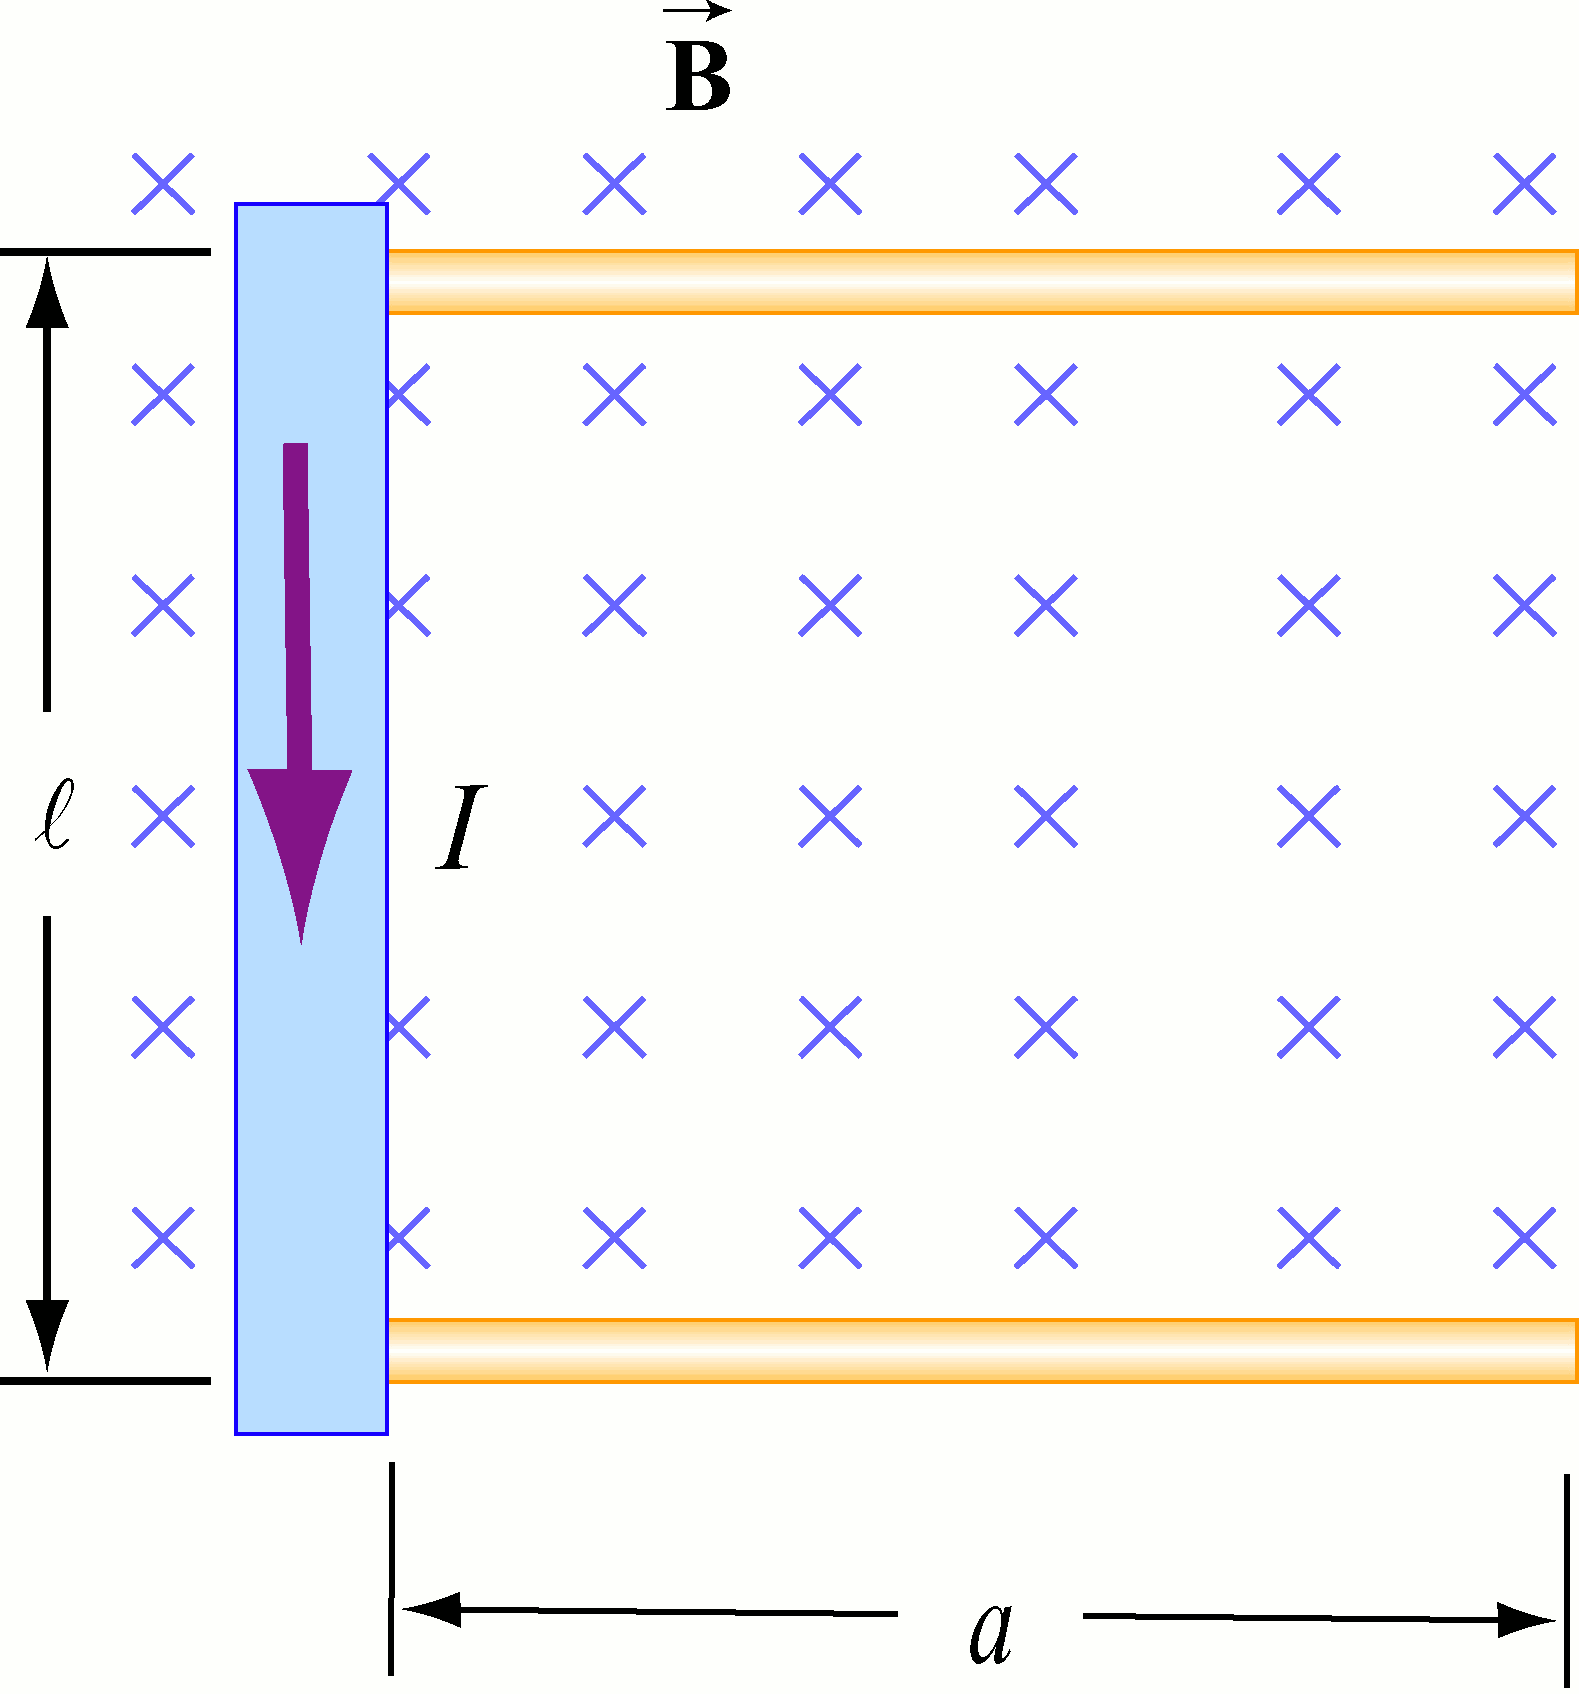
\includegraphics[width=0.33\textwidth]{ps07_03}\end{center}
\section{Problem \thesection: }
  A wire of arbitrary shape which is confined to the $x-y$ plane carries a current $I$ from point A to point B in the plane. Show that if a uniform magnetic field $B$ perpendicular to the $x-y$ plane is present, the force that the wire experiences is the same as that which would be felt by a wire running straight from A to B.
\section{Problem \thesection: }
  Calculate the divergence of the magnetic field of a straight wire in Cartesian coordinates.
\section{Problem \thesection: }
  Consider a cube which has identical resistors with resistance $R$ along each edge, as shown below.
  \begin{center}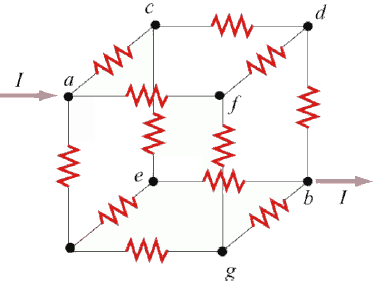
\includegraphics[width=0.33\textwidth]{ps07_06}\end{center}
  Find the equivalent resistance between points $a$ and $b$.
\section{Problem \thesection: }
  \begin{center}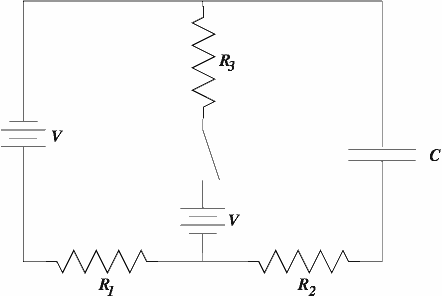
\includegraphics[width=0.5\textwidth]{ps07_07}\end{center}
  Suppose that the capacitor is initially charged.  The switch is closed at $t = 0$.  Find the current $I_{R_3}(t)$ through resistor $R_3$ (i.e., in the middle branch) as a function of time, and the charge in the capacitor $Q(t)$.  (Hint: this problem can be simplified greatly using Th\'evenin.  Compute $Q(t)$ first.)
\section{Problem \thesection: }
  Consider two parallel plates as shown in the sketch.  They each have a surface area $A$ and are separated by a distance $s$ that is small compared to the dimensions of the plate.  The top plate has a charge $+2Q$ deposited on it, while the bottom plate has charge $-Q$ deposited on it.  The two plates are not connected in any way.  For the purposes of this problem, assume that the charge densities are uniform on both surfaces of both plates, and ignore edge effects.
  \begin{center}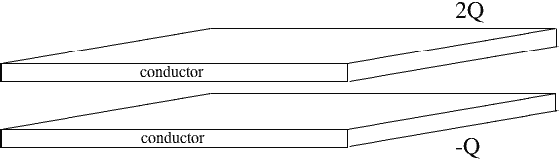
\includegraphics[width=0.75\textwidth]{ps07_08}\end{center}
  \begin{enumerate}[(a)]
    \item Find $\vec E$ between the two plates.
    \item Find the surface charge densities on the top and bottom faces of each of the two plates.
    \item Find $\vec E$ just above the top plate and just below the bottom plate.
    \item Show explicitly that the jump in $\vec E$ across each of the two plates is equal to $4\pi \sigma \hat n$ where $\sigma$ is the total surface charge density on that plate.
  \end{enumerate}
\end{document}
